%%%%%%%%%%%%%%%%%%%%%%%%%%%%%%%%%%%%%%%%%%%%%%%%%%%%%%%%%%%%%%%%%%%%%%%%%%%%%%%%
%                           RESULTS EXPERIMENTS CHAPTER 7                      %
%%%%%%%%%%%%%%%%%%%%%%%%%%%%%%%%%%%%%%%%%%%%%%%%%%%%%%%%%%%%%%%%%%%%%%%%%%%%%%%%
This section presents experimentations of the \gls{gv} in different contexts, namely (Exp.~1) when the implementation embeds no counter-measure, (Exp.~2) when traces are de-synchronized and (Exp.~3) when Boolean secret-sharing is applied.
The methods used to train the \glspl{cnn}, to tune their \glspl{hp} and to generate the \gls{gv} have been presented in \autoref{sec:method_cosade}.

\subsection{Application Without Counter-measure}
\label{sec:no_mask_no_desynchro}

\begin{table}
    \centering
    \caption{Settings and results of Exp.~1}
	\label{table:no_mask_no_desync}
    \begin{subtable}{0.49 \textwidth}
        \centering
        \caption{Architecture \glspl{hp}.}
        \begin{tabular}{l r}
            \toprule
            Parameter & Value \\
            \midrule
            \(n_2\) & 5 \\
            \(n_1\) & \{0, 1, 2\} \\
            \bottomrule
        \end{tabular}
        \label{table:no_mask_no_desync_left}
    \end{subtable}
    \begin{subtable}{0.49 \textwidth}
        \centering
        \caption{Performance metrics without counter-measure.}
        \begin{tabular}{l c r}
            \toprule
            \(n_1\) & Loss (bit) & \(\numTracesAttack(\MLmodel)\) \\
            \midrule
            0 & \(6.40\) & \(3.25\) \\
            1 & \(6.15\) & \(3\) \\
            2 & \(6.35\) & \(3.25\) \\
            \bottomrule
        \end{tabular}
        \label{table:no_mask_no_desync_center}
    \end{subtable}
\end{table}

In application context (Exp.~1) -- \ie{} no counter-measure -- several \glspl{cnn} have been trained with the architecture \glspl{hp} in \autoref{eq:vgg_archi_cosade} specified as listed in \autoref{table:no_mask_no_desync_left}. 
Since the random shares are here directly targeted -- \ie{} the masks are supposed to be known -- without re-combination -- thereby no dense layer -- should be required, according to the study of Benadjila \etal{}~\cite[Sec.~4.2.4]{prouff_study_2018}. 
The \gls{hp} \(n_1\) should therefore be null. 
However, to validate this intuition we let it vary in \(\{0,1,2\}\). 
The validation loss corresponding to these values is given in \autoref{table:no_mask_no_desync_center}, where \(\numTracesAttack(\MLmodel)\) denotes here the minimum number of traces required to have a \gls{ge} lower than \(1\).
Even if this minimum is roughly the same for the three different configurations, we selected the \emph{best} one 
-- \ie{} \(n_1=1\) -- for our \emph{best} \gls{cnn}  architecture. 
\autoref{fig:no_mask_no_desynchro_gv} presents the corresponding \gls{gv}, and \autoref{fig:no_mask_no_desynchro_snr} depicts the corresponding \gls{snr}.
It may be observed that the peaks obtained with \gls{gv} and \gls{snr} are identical: the highest point in the \gls{snr} is the second highest point in \gls{gv}, whereas the highest point in \gls{gv} is ranked \(7\)-th in the \gls{snr} peaks. 
More generally both methods target the same clock cycle (the \(19\)-th).
These observations validate the fact that our characterization method is relevant for an unprotected target.

\begin{figure}
    \centering
    \begin{subfigure}{0.49 \textwidth}
        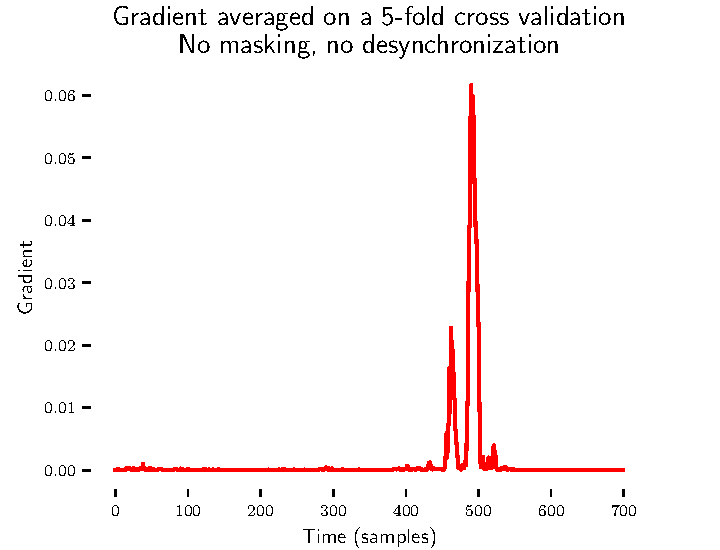
\includegraphics[width=\textwidth]{figures/ASCAD_700/no_mask_no_desynchro/VBP_n_dense_1_mean_review}
        \caption{\gls{gv} for the trained model with one dense layer, averaged over the validation traces.}
        \label{fig:no_mask_no_desynchro_gv}
    \end{subfigure}
    \begin{subfigure}{0.49 \textwidth}
        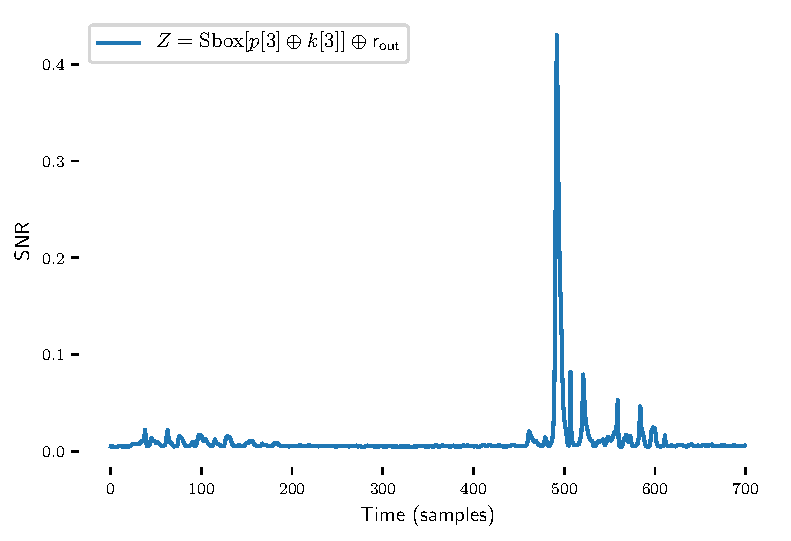
\includegraphics[width=\textwidth]{figures/ASCAD_700/snr_ascad_unmasked}
        \caption{The corresponding \gls{snr}.}
        \label{fig:no_mask_no_desynchro_snr}
    \end{subfigure}
	\caption{Case where no counter-measure is considered.}
    \label{fig:no_mask_no_desynchro}
\end{figure}
In addition to the \gls{gv} we also show in \autoref{fig:jacob_exp_1} the \gls{jacob} of the trained model.
Around the time coordinate 500 along the x-axis, some blue areas depict a high value in the matrix.
One may remark that those blue areas particularly appear for value of the sensitive variable -- along the  ordinates axis -- whose Hamming weight is one.
Since a high value in the \gls{jacob} implies a high sensitivity to slight changes in the input trace at the considered time coordinate, we may imagine that the trained \gls{cnn} is able to give a high confidence when expected to predict those values of the sensitive variable.
In other words, they are more distinguishable than the other values.
Although not a formal proof, this observation is coherent with a Hamming weight leakage model, where values of the target variable with low -- \eg{} 0 or 1 -- or high -- \eg{} 7 or 8 -- Hamming weight are more distinguishable than the others.
This example hence shows how the \gls{jacob} can bring additional insights compared to the gradient.

\begin{figure}[h]
    \centering
    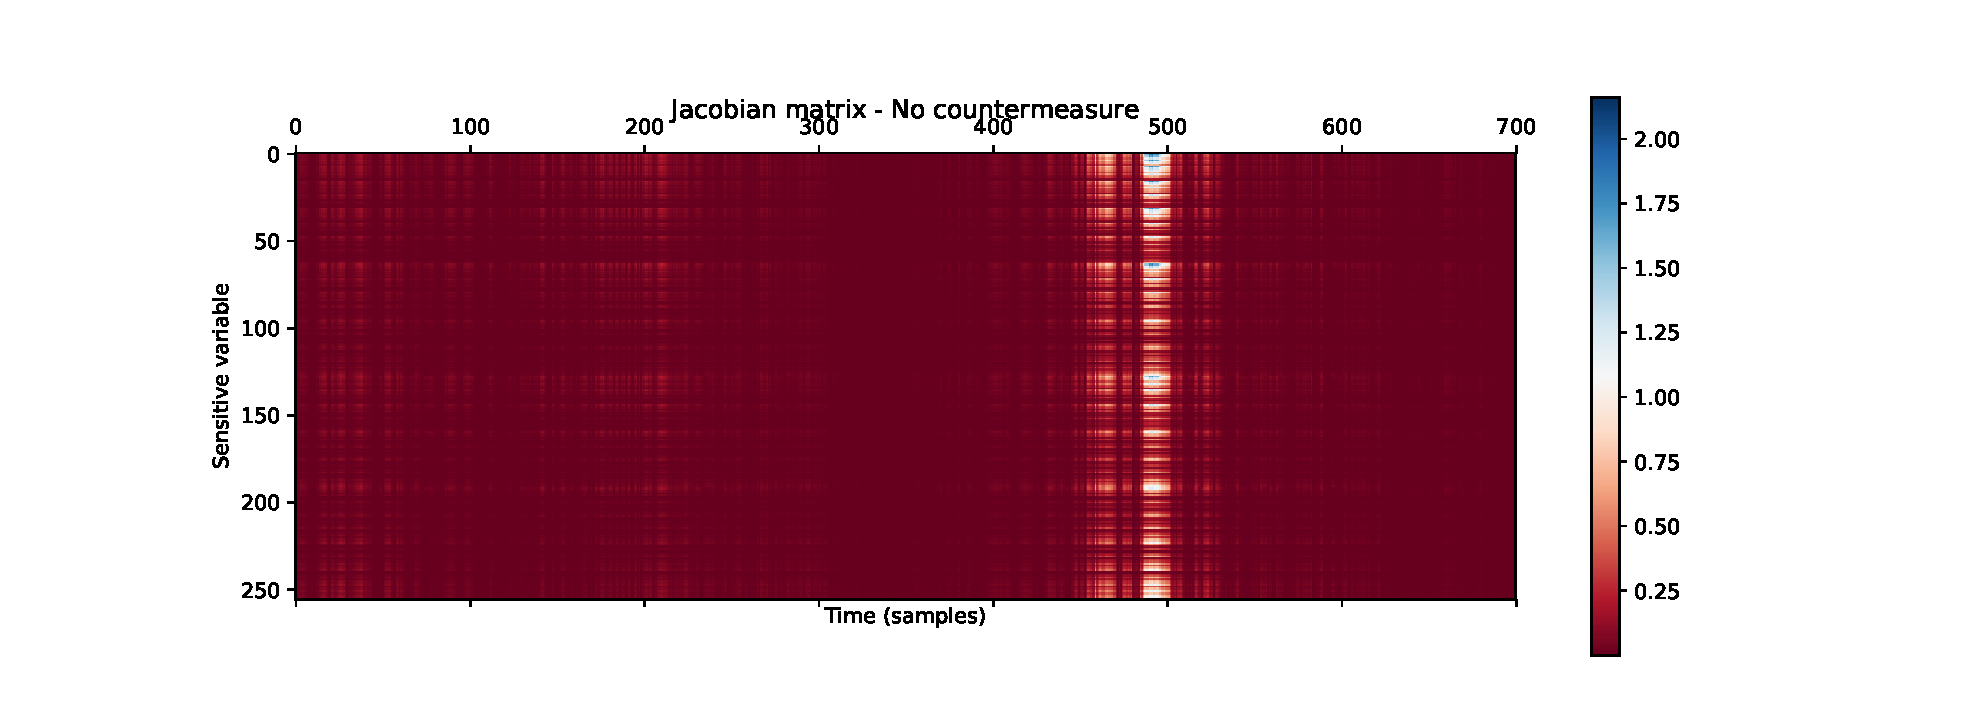
\includegraphics[width=\textwidth]{figures/ASCAD_700/no_mask_no_desynchro/jacob_n_dense_0_CV_0}
    \caption{\gls{jacob} for the best models in application context Exp.~1.}
    \label{fig:jacob_exp_1}
\end{figure}

\subsection{Application with an Artificial De-synchronization}
\label{sec:no_mask_with_desynchro}
\begin{table}
    \centering
    \caption{Settings and results of Exp.~2}
    \label{table:no_mask_with_desync}
    \begin{subtable}{0.49 \textwidth}
        \centering
        \caption{Architecture \glspl{hp}.}
        \begin{tabular}{l r}
            \toprule
            Parameter & Value \\
            \midrule
            \(n_2\) & 5 \\
            \(n_1\) & \{0, 1, 2\} \\
            \bottomrule
        \end{tabular}
        \label{table:no_mask_with_desync_left}
    \end{subtable}
    \begin{subtable}{0.49 \textwidth}
        \centering
        \caption{Performance metrics with de-synchronization.}
        \begin{tabular}{l c r}
            \toprule
            \(n_1\) & Loss (bit) & \(\numTracesAttack(\MLmodel)\) \\
            \midrule
            0 & \(6.64\) & \(4.0\) \\
            1 & \(6.46\) & \(3.6\) \\
            2 & \(6.90\) & \(5.4\) \\
            \bottomrule
        \end{tabular}
        \label{table:no_mask_with_desync_right}
    \end{subtable}
\end{table}

We now add a new difficulty by considering the case of de-synchronization as described in \autoref{sec:settings_cosade}.
The \gls{hp} grid is exactly the same as in \autoref{sec:no_mask_no_desynchro}, and the corresponding loss is given in \autoref{table:no_mask_with_desync_right}. 
Faced to misalignment, the considered architectures have still good performances, and the attacks succeeded in roughly the same number of traces than before. 
Interestingly, \autoref{fig:no_mask_with_desynchro} shows that the \gls{gv} succeeds in recovering the leakage localization while the \gls{snr} does not. 
Actually, the gradient averaged over the profiling traces \autoref{fig:no_mask_with_desynchro_gv_avg} shows that, instead of having a small number of peaks, a band is obtained whose width approximately equals the maximum quantity of shift applied in the traces, namely 100 points. 
Moreover, individual gradients in \autoref{fig:no_mask_with_desynchro_gv_single} bring a single characterization for each trace, enabling to guess approximately the shift applied to each trace.

\begin{figure}
    \centering
    \begin{subfigure}[]{0.49 \textwidth}
        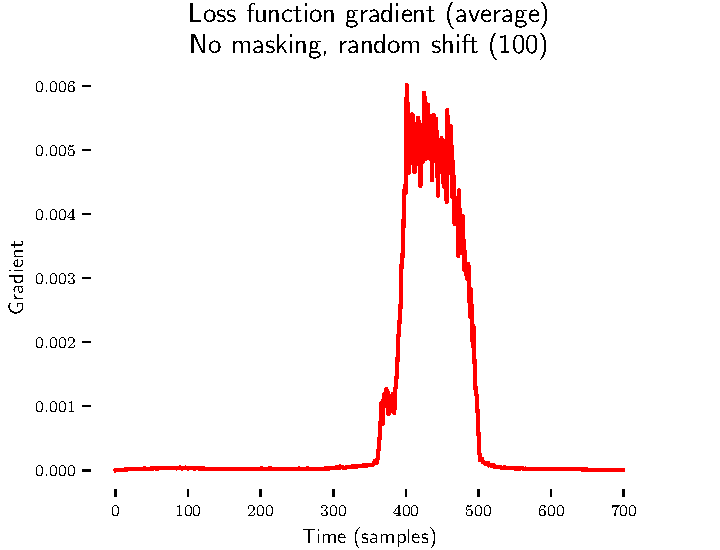
\includegraphics[width=\textwidth]{figures/ASCAD_700/no_mask_with_desynchro/grads_avg_n_dense_1_review}
        \caption{\gls{gv} averaged over all the traces.}
        \label{fig:no_mask_with_desynchro_gv_avg}
    \end{subfigure}
	\begin{subfigure}[]{0.49 \textwidth}
        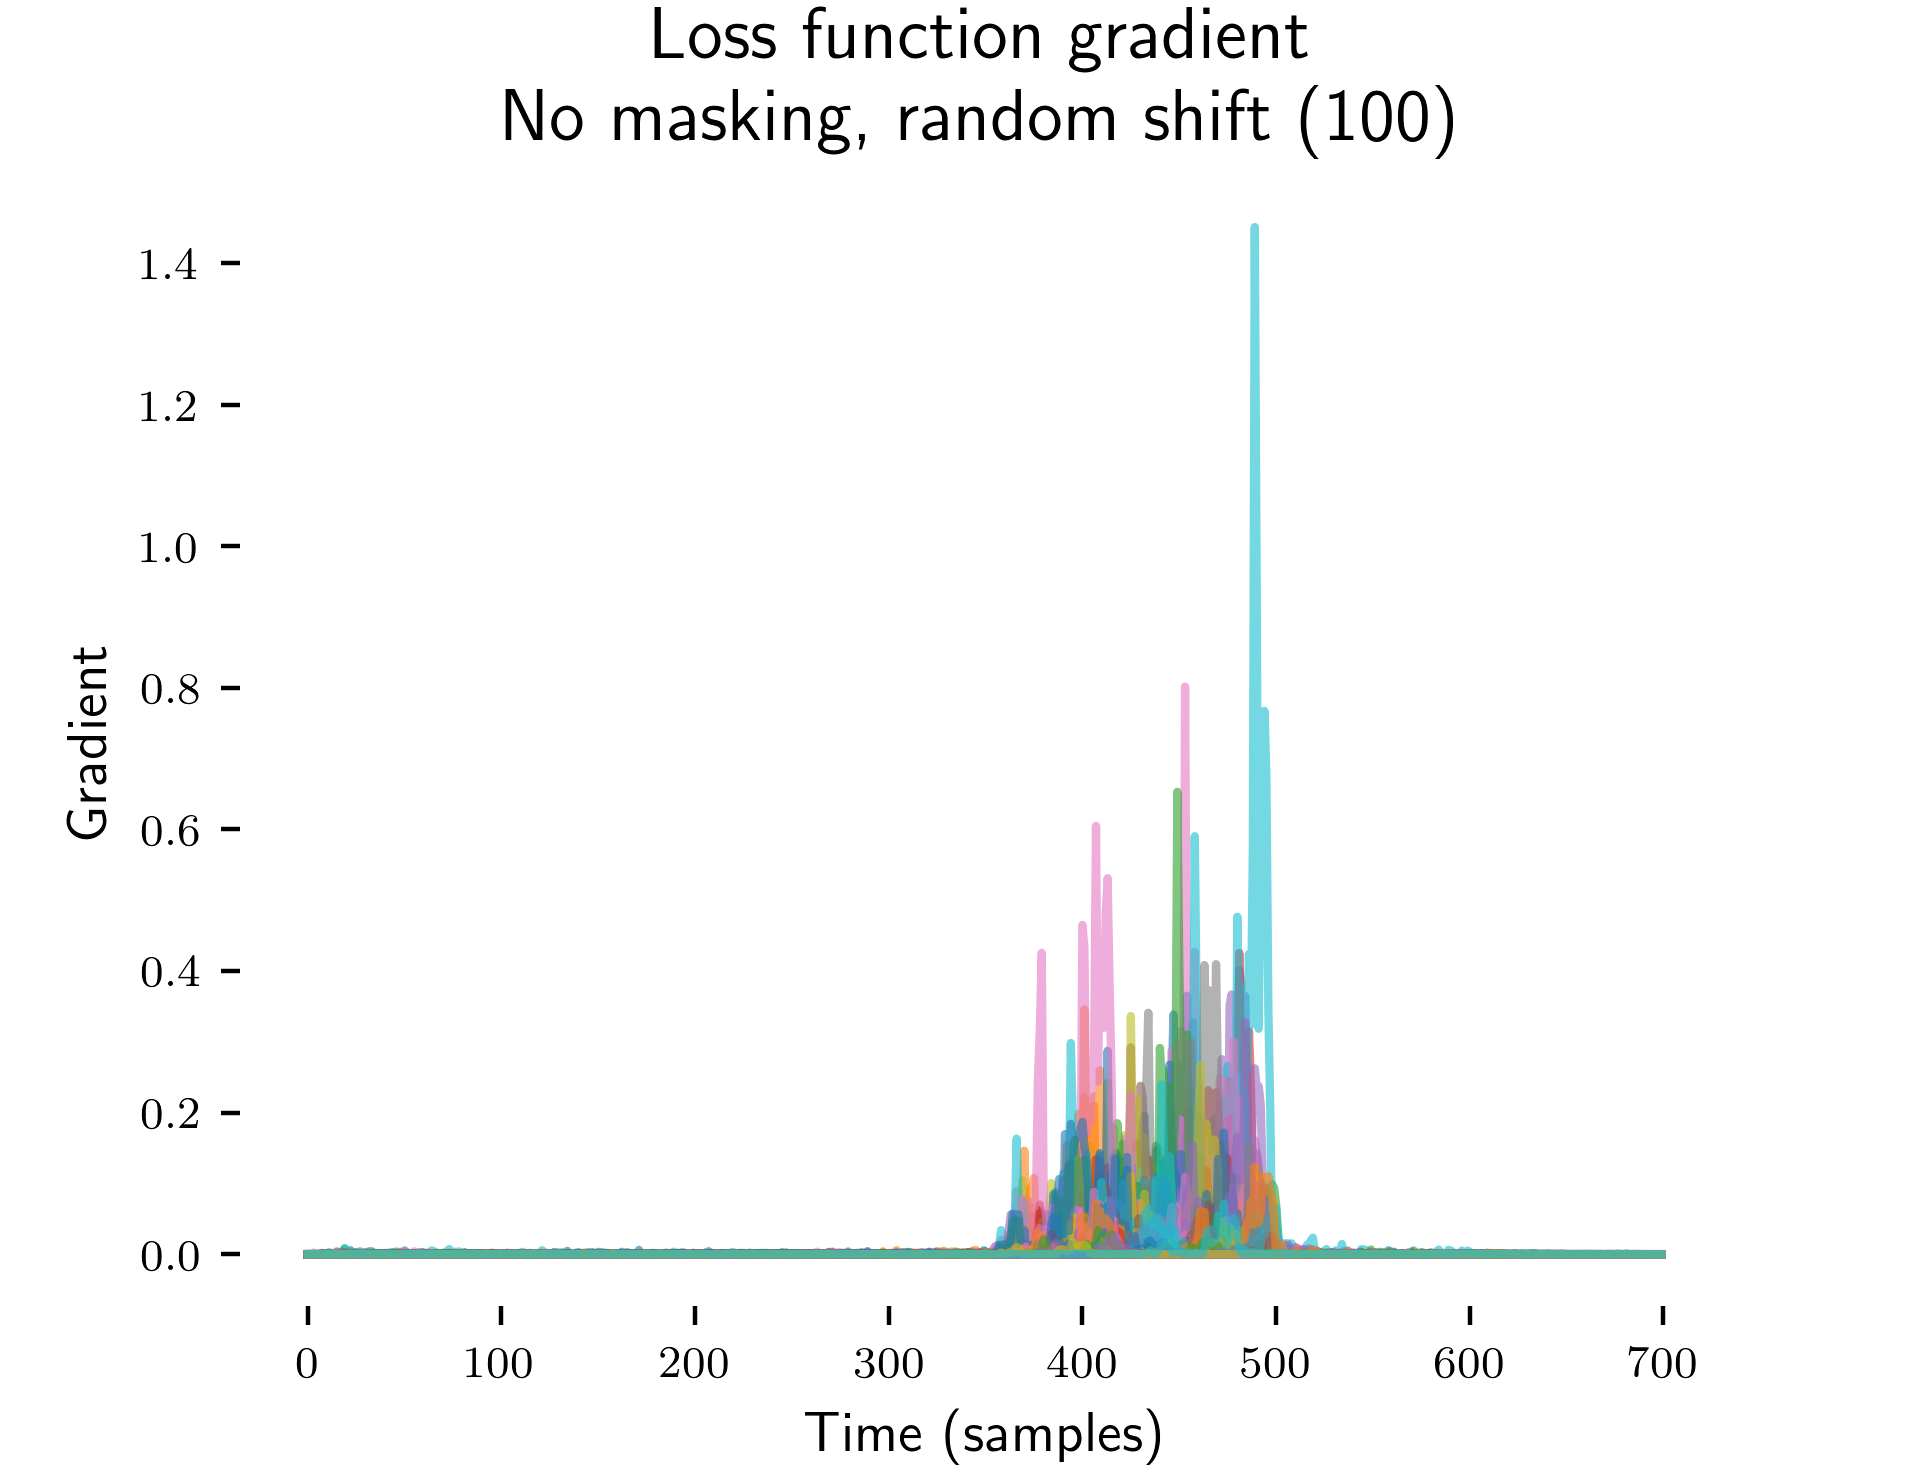
\includegraphics[width=\textwidth]{figures/ASCAD_700/no_mask_with_desynchro/all_grads_review.png}
        \caption{\gls{gv} for each trace separately.}
        \label{fig:no_mask_with_desynchro_gv_single}
    \end{subfigure}
    \begin{subfigure}[]{0.49 \textwidth}
        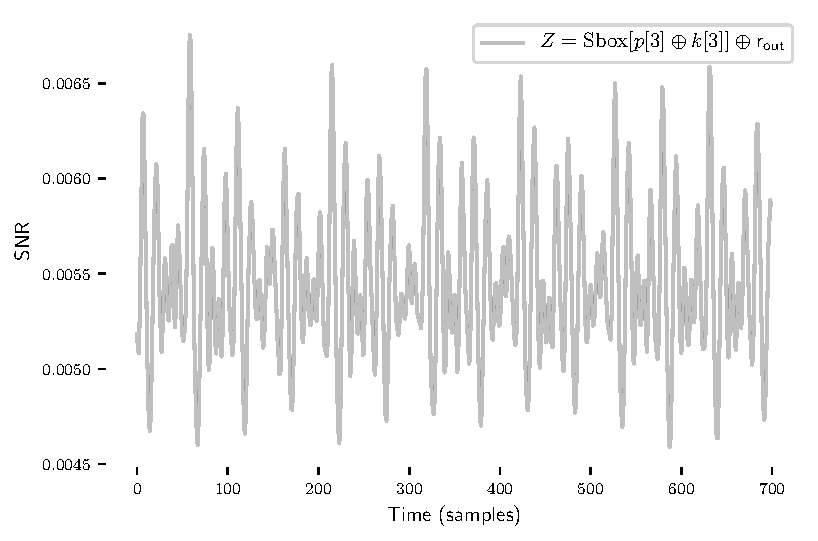
\includegraphics[width=\textwidth]{figures/ASCAD_700/snr_desync100}
        \caption{The corresponding \gls{snr}.}
        \label{fig:no_mask_with_desynchro_snr}
    \end{subfigure}
	\caption{Case where de-synchronization is considered.}
	\label{fig:no_mask_with_desynchro}
\end{figure}

\subsection{Application with a First Order Secret-Sharing}
\label{sec:with_mask_no_desynchro}
The next experiment concerns the application of \gls{gv} in presence of Boolean secret-sharing, namely the one implemented in the \gls{ascad} dataset.
Several model configurations have been tested which correspond to the \glspl{hp} listed in \autoref{table:ge_masking_hp}.
We eventually selected the \(8\) models that achieved the best efficiency, \ie{} the model \(\MLmodel(\cdot, \MLparam)\) with the lowest \(\numTracesAttack(\MLmodel)\) (\autoref{table:ge_masking_perf}).%
\footnote{
    Contrary to the convention taken in \autoref{sec:performance_metrics}, \(\numTracesAttack(\MLmodel)\) is here computed with respect to the \gls{ge}, as defined by \autoref{eq:eff_ge}.
}
 
\begin{table}
    \begin{subtable}{.49\textwidth}
        \centering
        \caption{Architecture \glspl{hp} -- bold values refer to the best choices.}
        \label{table:ge_masking_hp}
        \begin{tabular}{l r}
            \toprule
            Parameter & Value \\
            \midrule
            \(n_2\) & \{5, 6, \textbf{7}, 8\} \\
            \(n_1\) & \{\textbf{2}, 3\} \\
            \(\numFilters_0\) (first layer) & 10 \\
            \(\ksize\) & \{3, 5, \textbf{11}\} \\
            \bottomrule
        \end{tabular}
    \end{subtable}
    \begin{subfigure}{.49\textwidth}
        \centering
        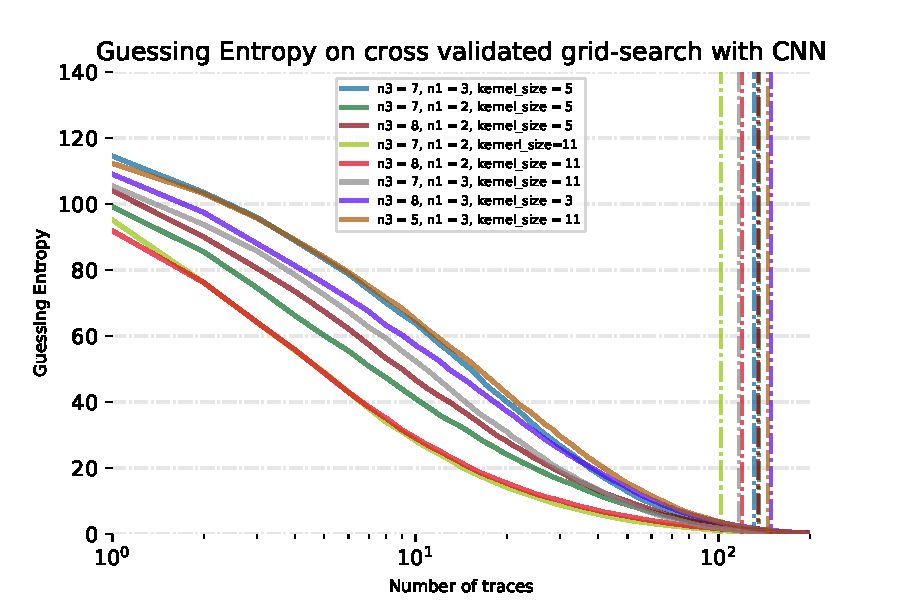
\includegraphics[width=\textwidth]{figures/ASCAD_700/with_mask_no_desynchro/GE_best_nodes}
        \caption{\gls{ge} for the \(8\) best architectures.}
        \label{table:ge_masking_perf}
    \end{subfigure}
    \caption{Results of Exp.~3 with Boolean secret-sharing.}
    \label{table:ge_masking}
\end{table}


For the selected architectures, our first attempt to use \gls{gv} did not give full satisfaction.
As an illustration, \autoref{fig:overfitting_peaks} presents it for one of the tested architectures -- averaged over the \(5\) folds of the cross-validation.
Indeed, it looks difficult to distinguish \glspl{poi}, \ie{} those identified by our \gls{snr} characterization, see \autoref{fig:vbp_masking_snr}, from \emph{ghost} peaks, \ie{} peaks \textit{a priori} independent of the sensitive target.
To explain this phenomenon, we decided to study the validation loss of the trained models.
\autoref{fig:overfitting_loss} presents it for one model and for each of the \(5\) cross-validation folds \(\mathrm{CV}_i$, $i\in \llbracket 0, 4 \rrbracket\).

\begin{figure}
    \centering
    \begin{subfigure}[]{0.49 \textwidth}
        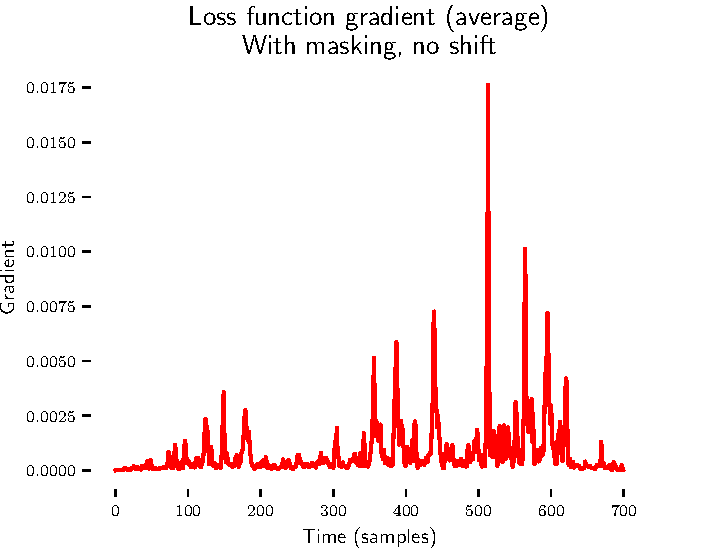
\includegraphics[width=\textwidth]{figures/ASCAD_700/with_mask_no_desynchro/VBP_Node_6191_without_early_stopping_review}
        \caption{\gls{gv} in presence of secret-sharing (without early-stopping).}
        \label{fig:overfitting_peaks}
    \end{subfigure}
    \begin{subfigure}[]{0.49 \textwidth}
        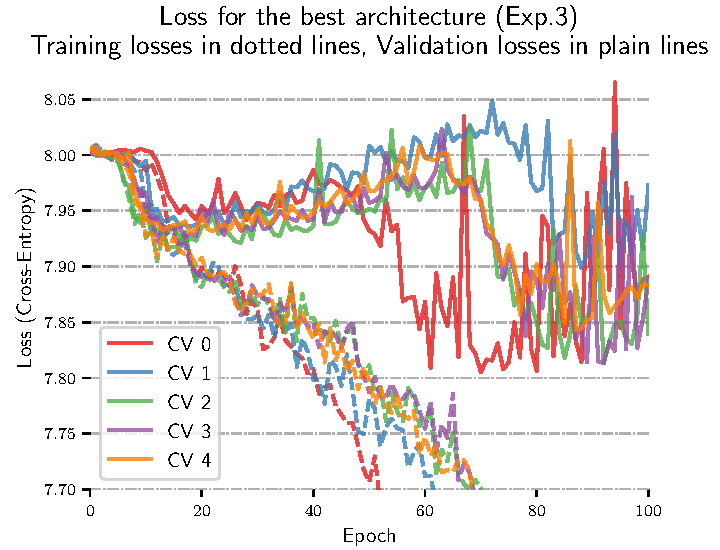
\includegraphics[width=\textwidth]{figures/ASCAD_700/with_mask_no_desynchro/Xent_Node_6191_review}
        \caption{Validation loss for each fold.}
        \label{fig:overfitting_loss}
    \end{subfigure}
	\caption{Explaining the ghost peaks.}
	\label{fig:overfitting}
\end{figure}

It may be observed in \autoref{fig:overfitting_loss} that the training and validation loss curves proceeded a fast big decrease after an initial plateau during the first \(15\) epochs.
After that, the validation loss starts increasing while the training loss still decreases.
After roughly \(50\) epochs, the validation loss goes on a regime with unstable results, but still higher than the training loss.
These observations are clues of over-fitting.%
\footnote{
    We recall the reader that an explanation of over-fitting has been given in \autoref{sec:results_exp}.
}
It means that the model exploits (non-informative) leakage not localized in the \glspl{poi} to memorize the profiling data and to improve the training loss.
Such a strategy should not generalize well on the validation traces.
As we are looking for models that implement a strategy that are generalizable on unseen traces, we propose to use a regularization technique called \emph{early-stopping}~\cite{goodfellow_deep_2017}: the training is stopped after a number of epochs called \emph{patience} -- in our case \(10\) -- if no remarkable decrease -- \ie{} up to a 
\emph{tolerance term}, \(0.25\) bits here -- is observed in the validation loss. 
With this slight modification, the previous architectures are trained again from scratch, and a better \gls{gv} is produced -- see \autoref{fig:vbp_masking_gv}.
As the main peaks are separated enough, an evaluator may conclude that they represent different leakages.

\begin{figure}
    \centering
    \begin{subfigure}{0.49 \textwidth}
        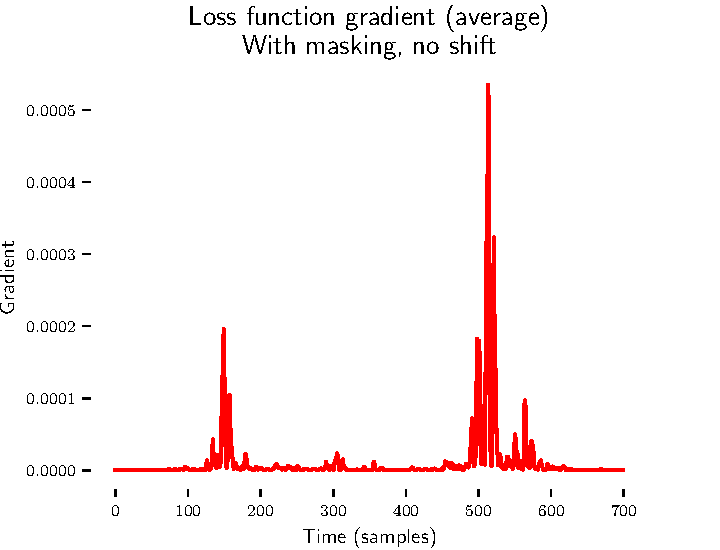
\includegraphics[width=\textwidth]{figures/ASCAD_700/with_mask_no_desynchro/VBP_Node_6191_review}
        \caption{\gls{gv}.}
        \label{fig:vbp_masking_gv}
    \end{subfigure}
    \begin{subfigure}{0.49 \textwidth}
        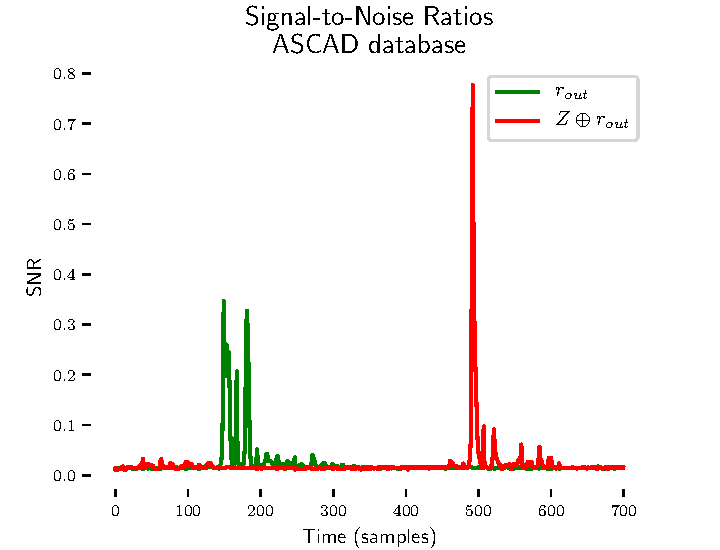
\includegraphics[width=\textwidth]{figures/ASCAD_700/snr_m_and_zxm}
        \caption{The corresponding \gls{snr} when taking \(\rout\) as a share.}
        \label{fig:vbp_masking_snr}
    \end{subfigure}
    \begin{subfigure}{0.49 \textwidth}
        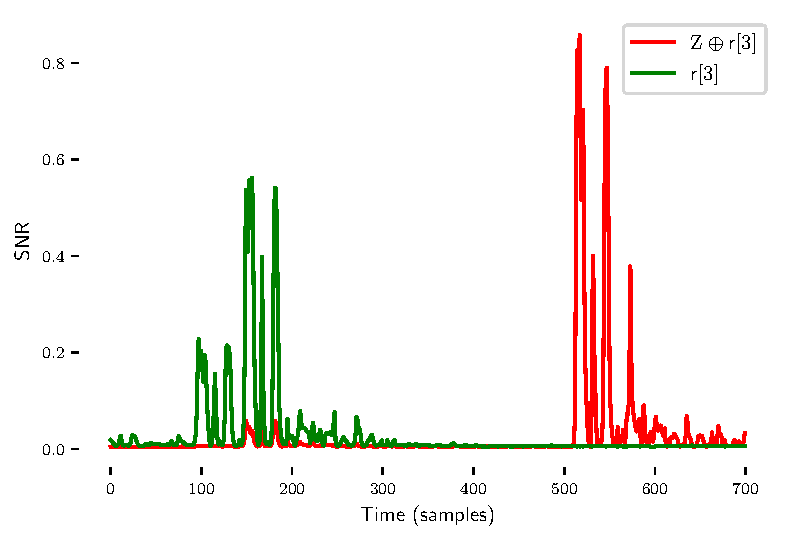
\includegraphics[width=\textwidth]{figures/ASCAD_700/snr_r3}
        \caption{The corresponding \gls{snr} when taking \(\M[3]\) as a share.}
        \label{fig:vbp_masking_snr_r3}
    \end{subfigure}
	\caption{Early-stopping is applied.}
	\label{fig:vbp_masking}
\end{figure}

\subsection{Comparison in the Context of Template Attacks}
\label{sec:comparison_with_snr}
A careful observation of \autoref{fig:vbp_masking} shows that the main peaks given by the \gls{gv} are not exactly aligned with those given by the \gls{snr} characterization -- performed under the hypothesis that the shares are known.
For \gls{gv}, the main peak appears at the points corresponding to the \(20\)-th clock cycle, which is one cycle after the one previously targeted by both the \gls{gv} and the \gls{snr} in the previous case where no counter-measure was considered -- see \autoref{sec:no_mask_no_desynchro}.
We validated that this phenomenon occurred for every successful visualization produced by \gls{gv}. 
Furthermore, concerning the peaks related to the mask leakage, the \gls{gv} only emphasizes one clock cycle (the \(6\)-th) whereas the \gls{snr} highlights two of them: the \(6\)-th and the \(7\)-th.
It implies that the \gls{gv} should not be taken as an exact equivalent to the \gls{snr}.

% Interpretation hypothesis
Actually, we found out a possible track of explanation to justify this slight shift by looking at the pseudo-code sketching the secret-sharing scheme of the \gls{ascad} database~\cite[Alg.~1]{prouff_study_2018}.
Indeed, the latter one emphasizes that another random variable forming a \(2\)-sharing of the output of \(\Sbox\), denoted as \(\mathsf{r}[3]\), is used in the scheme to protect the sensitive computation before and after applying the \(\sub{}\) operation, while the share \(\rout\) considered to compute the \gls{snr} in Figures \ref{fig:charac_ascad_snr} and \ref{fig:vbp_masking_snr} is used during the \(\sub{}\) operation.
By computing the \glspl{snr} of \(\Z \plusgf \mathsf{r}[3]\) and \(\mathsf{r}[3]\) in \autoref{fig:vbp_masking_snr_r3}, we remark that the peaks of \gls{snr} fit better with the peaks of \gls{gv} previously highlighted in the discussion.


Hence a question through this observation: does it have a sense for the trained \gls{cnn} to focus more on the leakages of the couple \((\Z \plusgf \mathsf{r}[3], \mathsf{r}[3])\) than on the leakages of the couple \((\Z \plusgf \rout, \rout)\)?
To give an answer, we decided to use our characterization method as a pre-processing for a Template Attack, and compare it to two pre-processing methods: \gls{snr} -- through \glspl{poi} selection -- and  \gls{pca} -- through dimensionality reduction.
The input dimension of the traces are reduced to \(2^n, n \in \{1, 2, 3, 4, 5\}\) points, based on the following methods:
\begin{itemize}
	\item \textbf{\gls{snr} strategy}: the \(2^{n-1}\) highest \glspl{poi} from the \gls{snr} of \(\rout\) and the \(2^{n-1}\) highest \glspl{poi} from the \gls{snr} of \(\Z \plusgf \rout\) are selected;
	\item \textbf{\gls{pca} strategy}: the \(2^n\) first components in a decreasing order of contribution are selected; 
	\item \textbf{\gls{gv} strategy}: the \(2^{n-1}\) highest \glspl{poi} from the \gls{gv} are selected from the area around the \(6\)-th clock cycle.
    Likewise, the other half comes from the peaks in the area around the \(20\)-th clock cycle.
\end{itemize}

\begin{remark}
    To make a fair comparison in the context of a first order secret-sharing, we assume that we know the shares during the characterization phase for \gls{snr}, so that we can localize the corresponding \glspl{poi}.
    Notice that we do not assume the mask knowledge neither during the profiling phase nor for the other strategies.
    Moreover, we do not use any re-combination function as described in \autoref{sec:PoIs} in none of the different strategies.

    Obviously, this scenario is not realistic as if one has access to the mask during characterization, then the latter one is very likely to be also available during the profiling phase.
\end{remark}


Once reduced, the traces are processed with a \gls{gta}, and the \gls{ge} is estimated.
The results are given on Figure~\ref{fig:ta_pois}. 
The plain curves denote the \gls{ge} for \gls{gv} whereas the dotted curves denote either \gls{ge} obtained with \gls{snr} (left) or \gls{pca} (right).

\begin{figure}
	\centering
    \begin{subfigure}{0.49 \textwidth}
        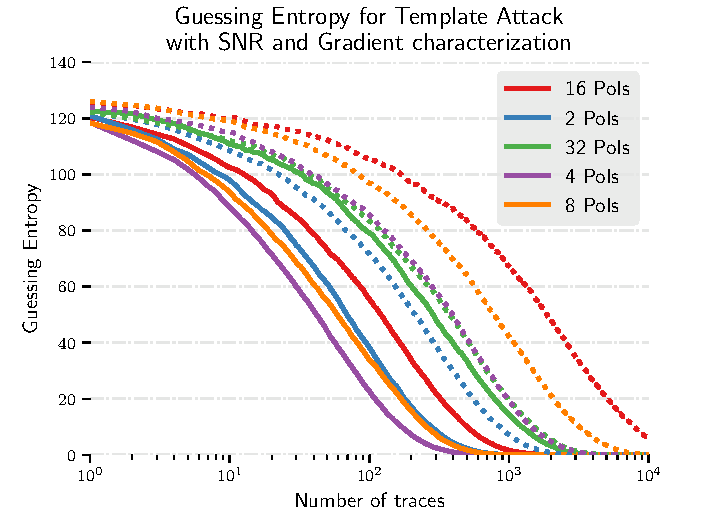
\includegraphics[width=\textwidth]{figures/ASCAD_700/with_mask_no_desynchro/GE_VBP_SNR_review}
        \caption{\ldots \gls{snr} based attacks.}
        \label{fig:ta_pois_snr}
    \end{subfigure}
    \begin{subfigure}{0.49 \textwidth}
        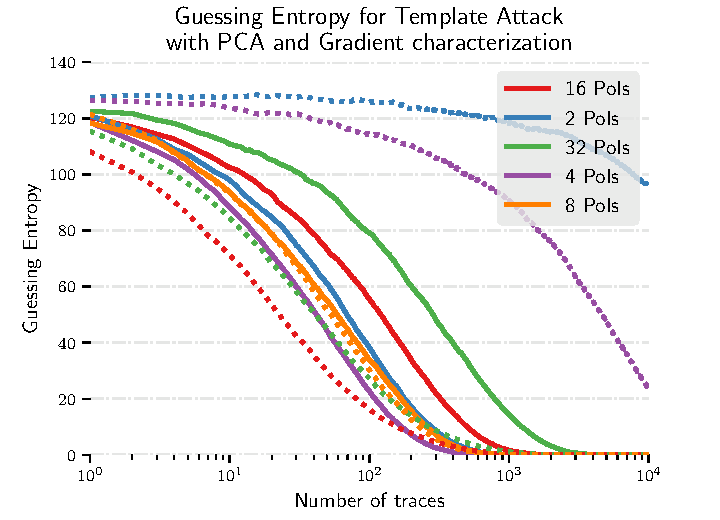
\includegraphics[width=\textwidth]{figures/ASCAD_700/with_mask_no_desynchro/GE_VBP_PCA_review}
        \caption{\ldots \gls{pca} based attacks.}
        \label{fig:ta_pois_pca}
    \end{subfigure}
	\caption{Comparison of the \gls{ge} for \gls{gv} based attacks in plain lines and, in dotted lines, \ldots}
	\label{fig:ta_pois}
\end{figure}

% Observations
From Figure~\ref{fig:ta_pois} we can observe several things:
\begin{itemize}
	\item Only a few \glspl{poi} from the \gls{gv} strategy are needed to get a successful attack.
	The optimal number of extracted \glspl{poi} is 4.
    Beyond that, the other \glspl{poi} bring more difficulty in the Template Attack than they bring new information (due to the increasing dimensionality).
	\item When the \gls{snr} strategy is applied, the optimal attack is done with 2 \glspl{poi} and the more \glspl{poi} are used, the less efficient are the attacks.
	This observation confirms that \gls{snr} selects relevant \glspl{poi} as expected. 
	However, when comparing the \gls{snr} and \gls{gv} strategies with a same number of \glspl{poi}, the latter one appears to be always better, except for 32 \glspl{poi} where both strategies seem equal.
	\item The \gls{pca} strategy does not work well for the two or four first extracted components.
    However, when considering eight components and above, it achieves an efficiency as good as the \gls{gv} strategy, and even sometimes better.
	\item In any case, the Template Attacks need much more traces to get a \gls{ge} converging towards zero than the best \gls{cnn} attack presented in Table~\ref{table:ge_masking}.
\end{itemize}

% First conclusion
Based on the presented experiments, we may draw several conclusions on the \gls{gv} efficiency.
First of all, it seems to be an accurate characterization method, almost always much better than that based on an \gls{snr}.
This first conclusion enables to answer the question previously asked: the targeted \glspl{poi} in \gls{gv} are relevant leakages and the couple of shares \((\Z \plusgf \mathsf{r}[3], \mathsf{r}[3])\) leaks more informative clues in the traces about the sensitive variable \(\Z\) than the couple of shares \((\Z \plusgf \rout, \rout)\).
Actually, this finding is not very surprising, since it could have been deduced from the \glspl{snr} computed by Benadjila \etal{} when presenting the \gls{ascad} database~\cite{prouff_study_2018}.
However, since the knowledge of the random shares is not required to train the \gls{cnn}, the attacker does not have to previously decide which sensitive intermediate computation is the most likely to lead to the most efficient attack.

% Second conclusion
Secondly, \gls{gv} can be used as a reliable dimensionality reduction pre-processing in presence of counter-measures, even more reliable than \gls{pca} in our cases where one makes a reduction to a very few dimensions (2 or 4).
However, this conclusion has a minor interest, as the \gls{gv} seen as a pre-processing method is done \textit{post-mortem}, and the training of a \gls{cnn} model did not suffer from a high dimensional input.

% Weakness
Last, but not least, the \gls{gv} method unfortunately faces a drawback: if the trained \gls{cnn} overfits, then the \gls{gv} might suffer from the presence of ghost peaks.
That is why the overfitting must be carefully monitored.
In this sense, visualizing the gradient can hopefully help to assess whether it is the case or not.